\newpage
\section{Aplikacja główna}
\paragraph{}
Głównym założeniem aplikacji w Unity jest stworzenie wirtualnego świata składającego się z wizualizacji dwóch ścian oraz elementów znajdujących się na nich. Po wyznaczonych elementach poruszać się będą aktorzy, czyli postacie gry.

\subsection{Świat gry}
\paragraph{}
Na wizualizacji dwóch ścian znajdują się przeszkody, czyli wirtualne platformy zbudowane z prostopadłościanów. Część z nich nakłada się na rzeczywiste elementy - na przykład rura ciepłownicza. Na platformach się elementy aktywne, które reaguję na interakcje z aktorem. Aby pokonać przeszkodę, będzie musiał on wykonać jedną z dostępnych w danej chwili akcji (np. rozbicie szklanego elementu czy też wykopanie).

\begin{center}
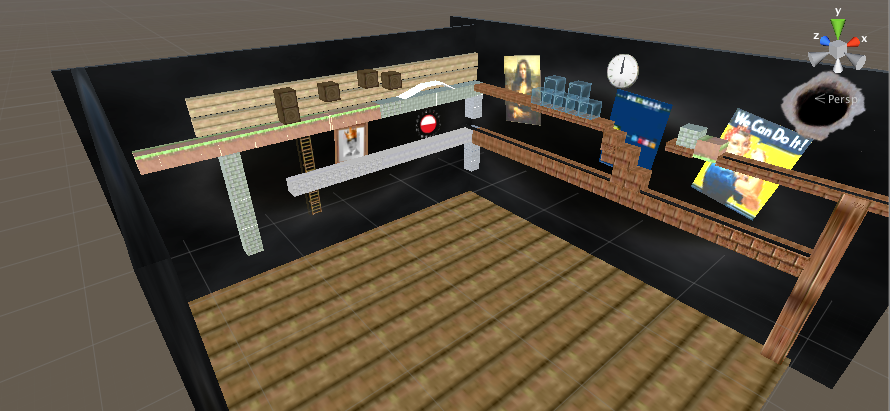
\includegraphics[width=1\textwidth]{images/swiatgry.png}
\captionof{figure}{
Model w środowisku Unity
}
\small {źródło: własne }
\end{center}


\subsection{Aktorzy}
\paragraph{}
Aktor to element interaktywny w grze. Podczas jej inicjalizacji aktor (prefabrykat z gotowym trójwymiarowym modelem) zaczyna się poruszać w jednym kierunku. Zadaniem gracza (za pomocą kontrolera) jest nadanie jednej z wielu umiejętności, tak aby aktor mógł przejść z miejsca startu do końca planszy.

Zaimplementowane możliwośći aktora to:

\begin{itemize}
	\item wykopanie elementu
	\item spadochron - swobodne spadanie
	\item rozbicie za pomocą kilofa elementu
	\item umiejętność skakania
	\item umiejętność zatrzymania się i ponownego swobodnego przechodzenia
	\item reset - powrót do pozycji startowej
\end{itemize}

\begin{lstlisting}[language=CSharp]
public static Vector3 lemmingPosition = new Vector3 (1205.9F, 103.4F, -4996.9F);
private static Vector3 jumpSize = new Vector3 (0, 200F, 0F);
\end{lstlisting}
\captionof{lstlisting}{
	Konfiguracja pozycji początkowej i siły skoku
}

\begin{lstlisting}[language=CSharp]
public void SendInfo() {
	Network.SendMessage("hasax_"+this.hasAx);
	Network.SendMessage("hassh_"+this.hasSh);
	Network.SendMessage("hasdrabina_"+this.drabina);
	Network.SendMessage("isMove_"+this.isMove);
}
\end{lstlisting}
\captionof{lstlisting}{
	Przykład wysyłania komunikatów do serwera
}

\paragraph{}
Podczas tworzenia nowej instancji klasy Aktora zapisywana ona jest do listy statycznej wszystkich dostępnych na daną chwilę obiektów (podczas usunięcia z planszy element również znika z listy). Ma to na celu możliwość implementacji w kontrolerze możliwości wyboru aktywnego aktora.

\begin{lstlisting}[language=CSharp]
public static void GetNext() {
Debug.Log ("get next");
if (Lemming2.activeEl == null) {
	Lemming2.activeEl = Lemming2.lista [0];
} else {
	int i = Lemming2.lista.IndexOf(Lemming2.activeEl);
	if (i < Lemming2.lista.Count - 1) {
		Lemming2.activeEl = Lemming2.lista [i + 1];
	} else {
		Lemming2.activeEl = Lemming2.lista [0];
	}
}

Lemming2.activeEl.SendInfo ();
}
\end{lstlisting}
\captionof{lstlisting}{
	Wybór aktywnego aktora.
}

\paragraph{}
Każdy z aktorów posiada detekcję kolizji z innymi elementami za pomocą nadpisania wbudowanych metod w środowisko Unity. Są to: OnTriggerEnter, OnTriggerExit, OnCollisionEnter, OnCollisionExit. Kolizja od triggera, różni się tym, iż metody OnCollsion współpracują tylko z elementami, które posiadają zaimplementowaną fizykę (np. spadający element platformy), natomiast trigger to można być dowolny element, nie posiadający ,,ciała'' (np. ściana).

\paragraph{}
W celu uproszczenia detekcji kolizji z innymi elementami wprowadzono czarne prostopadłościany emitujące rzeczywiste ściany. Są one koloru czarnego, dzięki temu projektor emitujący obraz w tych miejscach nie wyśle światła widzialnego. Natomiast dzięki takiemu zabiegowi możliwe jest zamodelowanie w środowisku unity kolizji z rzeczywistymi elementami.

\begin{center}
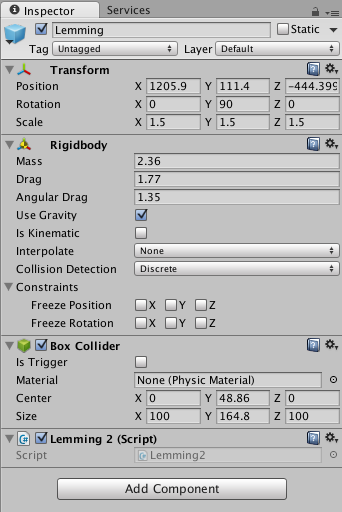
\includegraphics[width=1\textwidth]{images/aktor.png}
\captionof{figure}{
Konfiguracja aktora
}
\small {źródło: własne }
\end{center}

\subsection{Prefabrykaty}
\paragraph{}
W Unity możliwe jest używanie prefabrykatów (Prefabs \footnote{http://docs.unity3d.com/Manual/Prefabs.html}). Są obiekty lub grupy obiektów, które służą do wielokrotnego wykorzystywania. W Projekcie założono, że wszystkie reużwalne komponenty (dziedziczone pomiędzy scenami) będą prefabrykatami.

Dodatkowo aktorzy gry (generowane dynamicznie) są również prefabrykatami. Instancje aktora są tworzone podczas działania aplikacji.

\subsubsection{Kamery}
\paragraph{}
Ważnym elementem gry są wirtualne kamery. To z nich renderowane jest ujęcie, czyli obraz gry. W projekcie zastosowano dwie kamery. Podczas konfiguracji uruchomieniowej należy ustawić by każda z kamer była wyświetlana na oddzielnym źródle obrazu (monitor, projektor). Dzięki temu projekt można uruchomić na dwóch prostopadłych ścianach.
\paragraph{}
Jako tło sceny wybrano jednolity kolor czarny, ponieważ ten kolor nie jest prezentowany podczas projekcji. Światło z projektora jest w tym miejscu znikome, wręcz niewidoczne. Stosując taki prosty zabieg można łączyć elementy rzeczywiste (np. rura czy inne elementy stałe znajdujące się w laboratorium) z wirtualną rzeczywistością.

\begin{center}
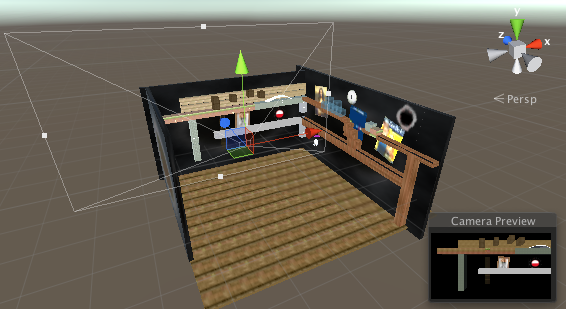
\includegraphics[width=1\textwidth]{images/kamera1.png}
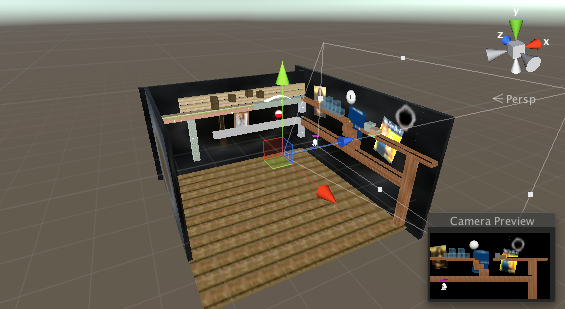
\includegraphics[width=1\textwidth]{images/kamera2.png}
\captionof{figure}{
Ujęcie wirtualnych kamer
}
\small {źródło: własne }
\end{center}

\paragraph{}
Środowisko Unity domyślnie nie ma włączonej opcji wspierania wielu kamer jednocześnie. Do opisywanego prefakbrykatu należy dodać abstrakcyjny GameObject z poniższym prostym skryptem, który przy uruchomieniu skompilowanej gry sprawdza dostępność sprzętową ekranów.

\begin{lstlisting}[language=CSharp]
using UnityEngine;
using System.Collections;

public class DisplayScript : MonoBehaviour
{
	void Start()
	{
		Debug.Log("displays connected: " + Display.displays.Length);
		if (Display.displays.Length > 1)
			Display.displays[1].Activate();
		if (Display.displays.Length > 2)
			Display.displays[2].Activate();
	}
}
\end{lstlisting}
\captionof{lstlisting}{
	Prosta aktywacja ekranów
}

\paragraph{}
Podczas testów uruchomieniowych przy dwóch kamerach występował problem z wydajnością karty graficznej. Zwłaszcza gdy do komputera podłączano dwa zewnętrzne ekrany po złączach cyfrowych (np. HDMI, DisplayPort, DVI). Finalnie problem rozwiązano wydajniejszym komputerem, jednakże pośrednim rozwiązaniem było użycie portu VGA, który jest mniej obciążający dla karty graficznej.

\subsubsection{Światło}
\paragraph{}
Kolejny prefabrykat stworzono by zachować spójność w oświetleniu trójwymiarowej sceny. Służy on do zgrupowania wszystkich źródeł wirtualnego światła. Jest to element bez zawartej logiki biznesowej. Stworzono go w celu zachowania porządku w projekcie.


\subsection{SocketIO}
\paragraph{}
Jest to prefabrykat dostarczony jako komponent implementacji Socket.io w bibliotece Asset Store. Jest on udostępniony na licencji Open Source.  Musi być on umiejscowiony w każdej scenie, która korzysta z połączenia sieciowego. Umiejscowienie jest dowolne, gdyż jest to prefabrykat abstrakcyjny (nie posiada graficznej reprezentacji w trójwymiarowym modelu). W prefabrykacie wywołano skrpyt SocketIOComponent, który odpowiada za inicjalizacje komunikacji sieciowej.

\subsubsection{Network}
\paragraph{}
Jest to kolejny prefabrykat abstrakcyjny, który służy do uruchomienia klasy Network odpowiadającej za implementacje metod służących do dwustronnej komunikacji.
Prefabrykat ten jest nierozerwalnie złączony z SocketIO, gdyż bezpośrednio korzysta z metod dostarczonych przez tą bibliotekę.


\begin{lstlisting}[language=CSharp]
private SocketIOComponent socket;

// Use this for initialization
void Start () {
	GameObject go = GameObject.Find("SocketIO");
	socket = go.GetComponent<SocketIOComponent>();

	socket.On("open", InitGame);
	socket.On("button", Button);
}
\end{lstlisting}
\captionof{lstlisting}{
	Inicjalizacja skryptu
}

\paragraph{}
Na początku wyszukiwany jest obiekt gry o określonej nazwie, a następnie pobierany komponent, czyli obiekt klasy. Warto pamiętać, ze połączenie inicjalizowane jest już przy uruchomieniu, więc nie ma potrzeby ,,ręcznego'' zestawiania warstwy sieciowej.

Metoda On w klase SocketIOComponent odpowiada za nasłuchiwanie serwera. Jako pierwszy parametr przyjmuje ciąg znaków określający nazwę metody. Natomiast drugi to referencja do metody, która wywoła się podczas wywołania akcji o nazwie wynikającej z pierwszego parametru.

Na potrzeby łatwiejszego zarządzania zdarzeniami i uniknięcia błędów w nazwach przycisków stworzono enum, zawierający nazwy obsługiwanych przycisków. Wszystkie metody odpowiadające za komunikację, a zwłaszcza za zarządzanie stanami oraz nazwami przycisków powinny przyjmować w parametrze opisywany atrybut wyliczalny.

\begin{lstlisting}[language=CSharp]
using System;

namespace AssemblyCSharp
{
	public enum ButtonEnum
	{
		BUTTON1, BUTTON2, BUTTON3, BUTTON4, BUTTON5, BUTTON6, BUTTON7, BUTTON8, BUTTON9, BUTTON10
	}
}

\end{lstlisting}
\captionof{lstlisting}{
	Definicja przycisków.
}

\paragraph{}
Metoda zarejestrowana pod nazwą ,,open'' wywoła się przy udanym zestawieniu połączenia. Jest to najlepsze miejsce do wstępnej konfiguracji planszy gry oraz przycisków w kontrolerze.

\begin{lstlisting}[language=CSharp]
public void InitGame(SocketIOEvent e)
{
	socket.Emit("register_game");
	EnableButton(ButtonEnum.BUTTON1);
	SetText(ButtonEnum.BUTTON1, "Nazwa 1");
	DisableButton(ButtonEnum.BUTTON2);
}
\end{lstlisting}
\captionof{lstlisting}{
	Inicjalizacja komponentów
}

\paragraph{}
Powyższy przykład inicjalizacji pokazuje emitowanie akcji do serwera o nazwie ,,register\_game''. Służy on do zarejestrowania gry na serwerze. Od tego czasu wszystkie akcje z kontrolera (np. wciśnięcie przycisku) będzie emitowane do gry.
Dodatkowo ukazano wstępną konfigurację przycisków: Uaktywnienie przycisku pierwszego, ustawienie określonej nazwy oraz wyłączenie przycisku drugiego.

\subsubsection{Budowanie zapytania}

\begin{lstlisting}[language=CSharp]
public void SetText(ButtonEnum btn, string text) {
	Dictionary<string, string> dic = new Dictionary<string, string> ();
	dic.Add ("name", btn.ToString());
	dic.Add ("text", text);
	socket.Emit ("set_text", new JSONObject (dic));
}
\end{lstlisting}
\captionof{lstlisting}{
	Przykładowe zapytanie do gra - kontroler
}

\subsubsection{Replikator}
\paragraph{}
Replikator to komonent do tworzenia nowych instancji aktora. Ma na celu cykliczne dodawanie kolejnych obiektów aktora w miejsce startowe określone w jego klasie. Dodatkowo uruchamia on nasłuchiwanie akcji przycisków płynących od kontrolera i zamienia je na wywołania metod na obecnie wybranym elemencie - aktywnym aktorze.

\begin{center}
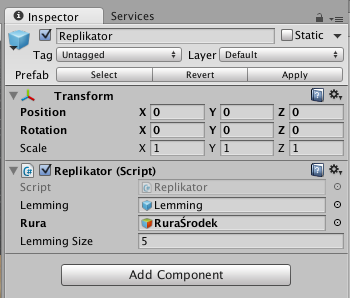
\includegraphics[width=0.7\textwidth]{images/replikator.png}
\captionof{figure}{
Konfiguracja replikatora
}
\end{center}

\begin{lstlisting}[language=CSharp]
...
public void Run () {
	StartCoroutine(Runner());

	NetworkManager.StartListening("button_left", Left);
	NetworkManager.StartListening("button_right", Right);
	NetworkManager.StartListening("button_kilof", Kilof);
	NetworkManager.StartListening("button_lopata", Lopata);
	NetworkManager.StartListening("button_jump", Jump);
	NetworkManager.StartListening("button_spadochron", Drabina);
	NetworkManager.StartListening("button_rotate", Rotate);
	NetworkManager.StartListening("button_startstop", Startstop);
	NetworkManager.StartListening("button_reset", Reset);
}

IEnumerator Runner() {
	while (lemmingCount < LemmingSize) {
		Create ();
		lemmingCount += 1;
		yield return new WaitForSeconds (secoundLimit);
	}
}
...
\end{lstlisting}
\captionof{lstlisting}{
	Uruchomienie replikatora
}

\begin{lstlisting}[language=CSharp]
...
void Left () {
	Lemming2.GetPrev ();
}

void Right () {
	Lemming2.GetNext ();
}

void Kilof () {
	if (Lemming2.activeEl) {
		Lemming2.activeEl.ToggleKilof ();
	}
}
...
\end{lstlisting}
\captionof{lstlisting}{
	Implementacja akcji
}

\subsection{Serwer komunikacyjny}
\paragraph{}
Jako technologię do obsługi połączeń zastosowano NodeJS. Obecnie jedyną zależnością zewnętrzną jest biblioteka Socket.IO \footnote{https://www.npmjs.com/package/socket.io}.
Jako manager zależności wybrano NPM. Jest on domyślnie dołączony do oprogramowania NodeJS. Aby pobrać zależności należy uruchomić polecenie ,,npm install'' w katalogu projektu.

\begin{lstlisting}[language=CSharp]
{
  "name": "server",
  "version": "1.0.0",
  "description": "",
  "main": "index.js",
  "author": "Kamil Warpechowski",
  "license": "GNU",
  "devDependencies": {
    "socket.io": "^1.4.6"
  }
}
\end{lstlisting}
\captionof{lstlisting}{
	Definicja zależności w projekcie
}

\paragraph{}
Głównym założeniem części serwerowej jest propagowanie wiadomości na linii kontroler - gra. Jednakże dzięki zastosowaniu Socket.IO możliwa jest obsługa wielu urządzeń jednocześnie. (np. dwóch kontrolerów). Dlatego też zastosowano mechanizm pokoi. Jest to grupowanie unikalnych identyfikatorów połączeń, co pozwala wysyłać komunikaty jednocześnie do wszystkich kontrolerów lub gier. Na potrzeby projektu wprowadzono limity (jedna gra, dwa kontrolery), jednakże w przyszłości jest możliwość dalszej rozbudowy.

\begin{lstlisting}[language=CSharp]
socket.on('register_controller', function () {
 if(io.sockets.adapter.rooms[CONTROLLER].length < 1) {
	console.log("register controller");
	socket.join(CONTROLLER);
 }
});

socket.on('register_game', function () {
   if(io.sockets.adapter.rooms[GAME]) {
	console.log("register game");
	socket.join(GAME);
   }
});
}
\end{lstlisting}
\captionof{lstlisting}{
	Grupowanie połączeń
}

\begin{lstlisting}[language=CSharp]
socket.on('enable_button', function (data) {
  console.log("enable_button", data);
  io.to(CONTROLLER).emit("enable_button", data);
});
\end{lstlisting}
\captionof{lstlisting}{
	Przykład propagacji komunikatu
}
\paragraph{}
W przyszłości możliwe jest przechowywanie stanu gry na poziomie serwera (każdy kontroler może przesłać unikalny identyfikator urządzenia).